\section{4. Tools, Resources, and
Interfaces}\label{tools-resources-and-interfaces}

This section groups the callable capability surface and the user-facing
layers that make that surface understandable.

\subsection{4.1 Tool registry and discovery
surface}\label{tool-registry-and-discovery-surface}

This subsection explains where the server's callable scope is registered
and how readers can inspect it quickly.

The routing spine for tools is
\href{https://github.com/chris-page-gov/mcp-geo/blob/fe862910da246ca77f374cfbe484985f5df4d316/server/mcp/tools.py\#L23-L123}{server/mcp/tools.py},
where explicit imports guarantee registration across environments, while
\href{https://github.com/chris-page-gov/mcp-geo/blob/fe862910da246ca77f374cfbe484985f5df4d316/docs/tool_catalog.md\#L1-L61}{docs/tool\_catalog.md}
gives the public catalog view and
\href{https://github.com/chris-page-gov/mcp-geo/blob/fe862910da246ca77f374cfbe484985f5df4d316/tools/registry.py}{tools/registry.py}
defines the shared registration model. This is the best place to orient
around breadth before drilling into a specific domain module.

Where to go:
\href{https://github.com/chris-page-gov/mcp-geo/blob/fe862910da246ca77f374cfbe484985f5df4d316/server/mcp/tools.py\#L1-L260}{server/mcp/tools.py},
\href{https://github.com/chris-page-gov/mcp-geo/blob/fe862910da246ca77f374cfbe484985f5df4d316/docs/tool_catalog.md\#L1-L61}{docs/tool\_catalog.md},
\href{https://github.com/chris-page-gov/mcp-geo/blob/fe862910da246ca77f374cfbe484985f5df4d316/tools/registry.py}{tools/registry.py},
and
\href{https://github.com/chris-page-gov/mcp-geo/blob/fe862910da246ca77f374cfbe484985f5df4d316/server/mcp/tool_search.py}{server/mcp/tool\_search.py}.

\subsection{4.2 Domain tool families and supporting
resources}\label{domain-tool-families-and-supporting-resources}

This subsection groups the domain modules so readers can find the right
problem space without reading every schema definition.

The
\href{https://github.com/chris-page-gov/mcp-geo/tree/fe862910da246ca77f374cfbe484985f5df4d316/tools}{tools/}
directory breaks cleanly into a few families: OS places and names in
\href{https://github.com/chris-page-gov/mcp-geo/blob/fe862910da246ca77f374cfbe484985f5df4d316/tools/os_places.py}{tools/os\_places.py},
\href{https://github.com/chris-page-gov/mcp-geo/blob/fe862910da246ca77f374cfbe484985f5df4d316/tools/os_places_extra.py}{tools/os\_places\_extra.py},
and
\href{https://github.com/chris-page-gov/mcp-geo/blob/fe862910da246ca77f374cfbe484985f5df4d316/tools/os_names.py}{tools/os\_names.py};
OS feature, map, and vector tile work in
\href{https://github.com/chris-page-gov/mcp-geo/blob/fe862910da246ca77f374cfbe484985f5df4d316/tools/os_features.py}{tools/os\_features.py},
\href{https://github.com/chris-page-gov/mcp-geo/blob/fe862910da246ca77f374cfbe484985f5df4d316/tools/os_maps.py}{tools/os\_maps.py},
\href{https://github.com/chris-page-gov/mcp-geo/blob/fe862910da246ca77f374cfbe484985f5df4d316/tools/os_vector_tiles.py}{tools/os\_vector\_tiles.py},
and
\href{https://github.com/chris-page-gov/mcp-geo/blob/fe862910da246ca77f374cfbe484985f5df4d316/tools/os_map.py}{tools/os\_map.py};
admin and route functions in
\href{https://github.com/chris-page-gov/mcp-geo/blob/fe862910da246ca77f374cfbe484985f5df4d316/tools/admin_lookup.py}{tools/admin\_lookup.py}
and
\href{https://github.com/chris-page-gov/mcp-geo/blob/fe862910da246ca77f374cfbe484985f5df4d316/tools/os_route.py}{tools/os\_route.py};
and ONS, NOMIS, and meta routing in
\href{https://github.com/chris-page-gov/mcp-geo/blob/fe862910da246ca77f374cfbe484985f5df4d316/tools/ons_data.py}{tools/ons\_data.py},
\href{https://github.com/chris-page-gov/mcp-geo/blob/fe862910da246ca77f374cfbe484985f5df4d316/tools/ons_geo.py}{tools/ons\_geo.py},
\href{https://github.com/chris-page-gov/mcp-geo/blob/fe862910da246ca77f374cfbe484985f5df4d316/tools/nomis_data.py}{tools/nomis\_data.py},
and
\href{https://github.com/chris-page-gov/mcp-geo/blob/fe862910da246ca77f374cfbe484985f5df4d316/tools/os_mcp.py}{tools/os\_mcp.py}.
Supporting static data and catalogs sit in
\href{https://github.com/chris-page-gov/mcp-geo/tree/fe862910da246ca77f374cfbe484985f5df4d316/resources}{resources/}.

Where to go:
\href{https://github.com/chris-page-gov/mcp-geo/tree/fe862910da246ca77f374cfbe484985f5df4d316/tools}{tools/},
\href{https://github.com/chris-page-gov/mcp-geo/tree/fe862910da246ca77f374cfbe484985f5df4d316/resources}{resources/},
\href{https://github.com/chris-page-gov/mcp-geo/blob/fe862910da246ca77f374cfbe484985f5df4d316/tools/os_map.py}{tools/os\_map.py},
\href{https://github.com/chris-page-gov/mcp-geo/blob/fe862910da246ca77f374cfbe484985f5df4d316/tools/os_apps.py}{tools/os\_apps.py},
\href{https://github.com/chris-page-gov/mcp-geo/blob/fe862910da246ca77f374cfbe484985f5df4d316/tools/ons_data.py}{tools/ons\_data.py},
and
\href{https://github.com/chris-page-gov/mcp-geo/blob/fe862910da246ca77f374cfbe484985f5df4d316/tools/os_route.py}{tools/os\_route.py}.

\begin{figure}
\centering
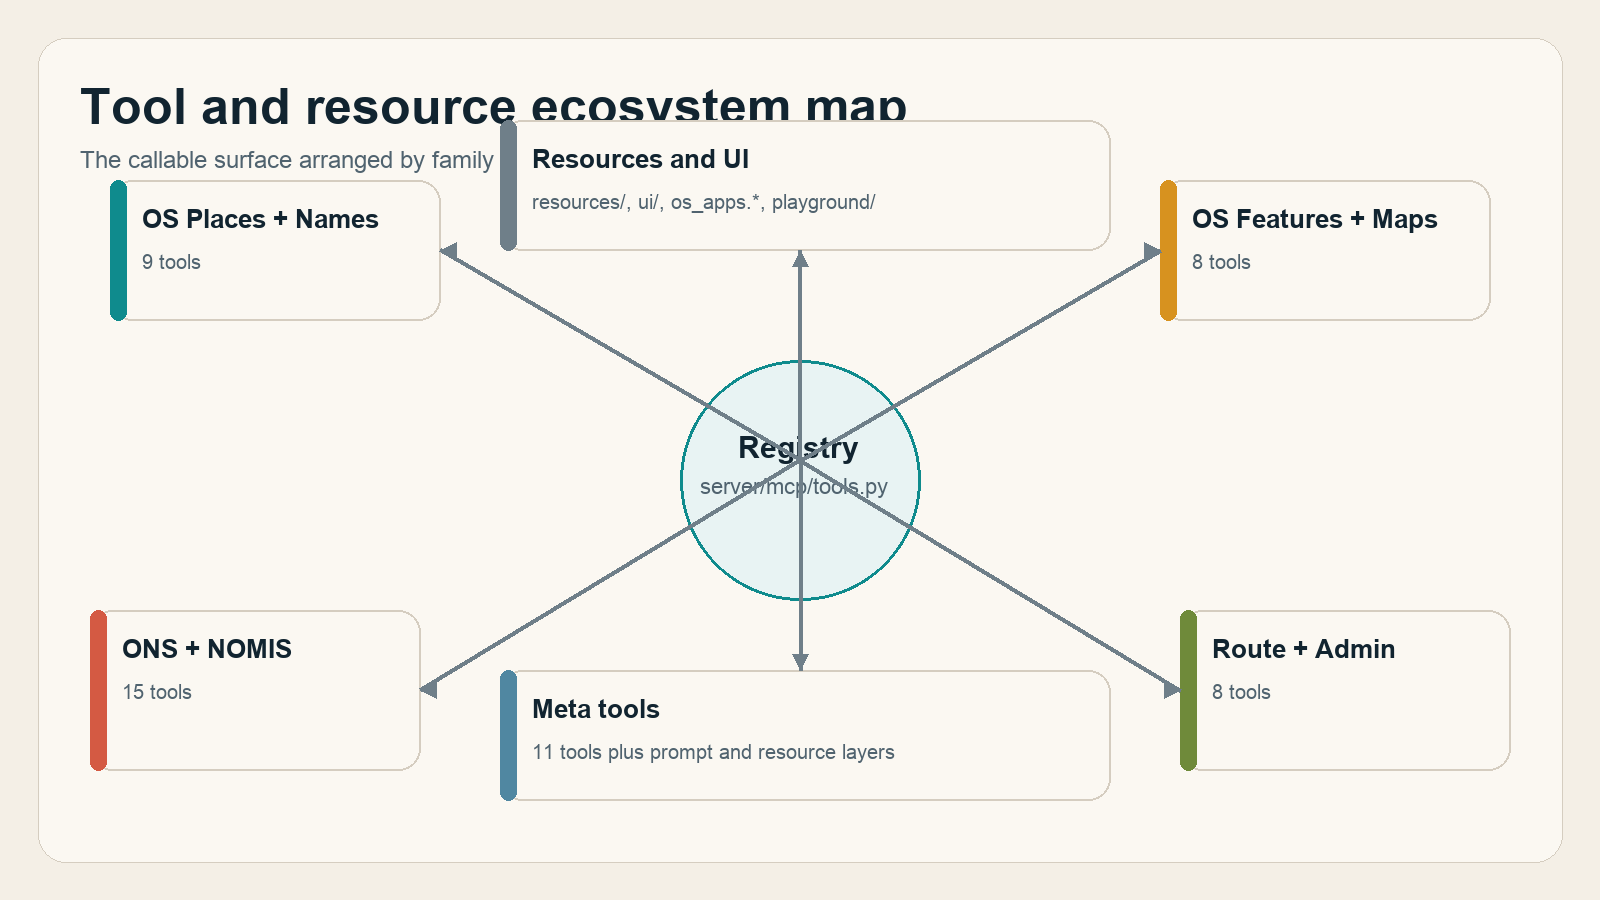
\includegraphics[width=0.96\linewidth,height=\textheight,keepaspectratio,alt={Figure F04. Tool and resource ecosystem map}]{figures/f04_tool_resource_ecosystem.png}
\caption{Figure F04. Tool and resource ecosystem map}
\end{figure}

Figure F04 gives the tool breadth in one picture, so the repo does not
have to be learned from schemas alone.

\subsection{4.3 UI surfaces, playground, and host-facing
views}\label{ui-surfaces-playground-and-host-facing-views}

This subsection points to the HTML and host-facing surfaces that let
readers see how MCP-Geo behaves in use rather than only in code.

The UI layer is split between
\href{https://github.com/chris-page-gov/mcp-geo/tree/fe862910da246ca77f374cfbe484985f5df4d316/ui}{ui/},
which holds individual HTML views such as
\href{https://github.com/chris-page-gov/mcp-geo/blob/fe862910da246ca77f374cfbe484985f5df4d316/ui/geography_selector.html}{geography
selector},
\href{https://github.com/chris-page-gov/mcp-geo/blob/fe862910da246ca77f374cfbe484985f5df4d316/ui/route_planner.html}{route
planner},
\href{https://github.com/chris-page-gov/mcp-geo/blob/fe862910da246ca77f374cfbe484985f5df4d316/ui/feature_inspector.html}{feature
inspector}, and
\href{https://github.com/chris-page-gov/mcp-geo/blob/fe862910da246ca77f374cfbe484985f5df4d316/ui/statistics_dashboard.html}{statistics
dashboard}, and
\href{https://github.com/chris-page-gov/mcp-geo/tree/fe862910da246ca77f374cfbe484985f5df4d316/playground}{playground/},
which provides the Svelte-based host inspection and test harness
surface. This is where the repo becomes visibly interactive.

Where to go:
\href{https://github.com/chris-page-gov/mcp-geo/tree/fe862910da246ca77f374cfbe484985f5df4d316/ui}{ui/},
\href{https://github.com/chris-page-gov/mcp-geo/tree/fe862910da246ca77f374cfbe484985f5df4d316/playground}{playground/},
\href{https://github.com/chris-page-gov/mcp-geo/blob/fe862910da246ca77f374cfbe484985f5df4d316/playground/src/App.svelte}{playground/src/App.svelte},
\href{https://github.com/chris-page-gov/mcp-geo/tree/fe862910da246ca77f374cfbe484985f5df4d316/playground/tests}{playground/tests/},
and
\href{https://github.com/chris-page-gov/mcp-geo/tree/fe862910da246ca77f374cfbe484985f5df4d316/output/playwright}{output/playwright/}.
